\subsection{1-reducibility of the ring $R_5$}

In the five color theorem, we used that every planar graph has a vertex with $\deg(v)\leq 5$. So far, we know that the cases $\deg(v) \leq 4$ are reducible when using four colors. If $\deg(v)=5$, we may add edges between the neighbors of $v$ to obtain the ring $R_5$. If $R_5$ were 0-reducible, then we would obtain our reduction by removing the vertex $v$. Therefore, the four color theorem would follow in the same fashion as the five color theorem.

Many have tried to show this, among which Alfred Kempe with his false proof. It must be hard (or require clever tricks) to prove that $R_5$ is 0-reducible. That is why Birhoff had proven in 1913 that $R_5$ is 1-reducible instead \cite{birkhoff}. So will we.

\begin{theorem}
    The ring $R_5$ is 1-reducible.
\end{theorem}

\begin{proof}
Let the planar graph $M+\confg$ with configuration $\confg=\core+R_5$ be arbitrary. Again, let the possible ring colorings be represented by

\begin{equation}
    \I = \Phi(M+S) \quad \text{and} \quad \II = \Phi(\core+S').
\end{equation}

Since $k=1$, we have colorings from both $S=R_5$ and $S=R_5+v$ in the sets of possible colorings $\I, \II$. Whether or not we need the reducer depends totally on the arbitrary choice of $M+\confg$. This is as expected, since there are many configurations that are in fact, 0-reducible.

Let us first consider the colorings contributed by the choice $S=R_5$, which means that we dont use a reducer.

\begin{figure}[!ht] 
    \centering
    \begin{tikzpicture}[mid arrow/.style={
        postaction={ decorate, decoration={ markings, mark=at position 0.6 with { \arrow[black]{>>} } } } }]
        \draw[fill=white] (-0.5, 0) ellipse (2cm and 1.5cm);
        \node (m) at (-1.7, 0) {$M$};
        \node at (-0.8, 0.8) {$R_5$};

        \node[circle, fill, scale=0.015cm] (l1) at (0, 1) { };
        \node[circle, fill, scale=0.015cm] (l2) at (0.9, 0.30) { };
        \node[circle, fill, scale=0.015cm] (l3) at (0.6, -0.77) {};
        \node[circle, fill, scale=0.015cm] (l4) at (-0.6, -0.77) {};
        \node[circle, fill, scale=0.015cm] (l5) at (-0.9, 0.30) {};
        \draw[mid arrow] (l1) -- (l2);
        \draw (l2) -- (l3) -- (l4) -- (l5) -- (l1);
    \end{tikzpicture}
    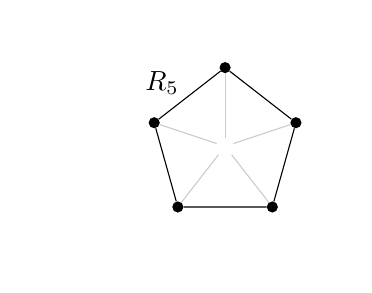
\begin{tikzpicture}[mid arrow/.style={
        postaction={ decorate, decoration={ markings, mark=at position 0.6 with { \arrow[black]{>>} } } } }]
        \draw[opacity=0] (-0.5, 0) ellipse (2cm and 1.5cm);
        \node at (-0.8, 0.8) {$R_5$};
        \node[inner sep=1mm] (c) at (0, 0) {$\core$};
        \node[circle, fill, scale=0.015cm] (l1) at (0, 1) { };
        \node[circle, fill, scale=0.015cm] (l2) at (0.9, 0.30) { };
        \node[circle, fill, scale=0.015cm] (l3) at (0.6, -0.77) {};
        \node[circle, fill, scale=0.015cm] (l4) at (-0.6, -0.77) {};
        \node[circle, fill, scale=0.015cm] (l5) at (-0.9, 0.30) {};

        \draw[opacity=0.2] (c) -- (l1);
        \draw[opacity=0.2] (c) -- (l2);
        \draw[opacity=0.2] (c) -- (l3);
        \draw[opacity=0.2] (c) -- (l4);
        \draw[opacity=0.2] (c) -- (l5);
        \draw (l1) -- (l2) -- (l3) -- (l4) -- (l5) -- (l1);
    \end{tikzpicture}
    \caption{The reductions $M+R_5$ and $\core+R_5$ ($\confg$).}
    \label{fig:ring5k0}
\end{figure}

Now we use the same trick as for the ring $R_4$. We may contract any two non-neighboring vertices of $R_5$ by Theorem \ref{thm:ringsarered}. This means that we get colorings of the form $a{*}{*}a{*}$ where the $a$-colored vertices got contracted. We dont know anything about the ${*}$-colors. Since there are 5 possible contractions of two vertices on $R_5$, we obtain 5 different colorings.

\begin{equation}
    \Phi^\star = \{ a{*}{*}a{*}, \quad {*}a{*}{*}a, \quad a{*}a{*}{*}, \quad {*}a{*}a{*}, \quad {*}{*}a{*}a{*} \}.
\end{equation}

Next we consider the colorings for $S=R_5+v$. We may freely choose our reducers $S$ and $S'$ here. We will try to guarantee a 3-coloring because they are simplest to work with. It also turns out that they are key to finding a common ring coloring, as we shall see. For this reason, we use a single vertex connected to all ring vertices for our reducers $S$ and $S'$. 

Note that the ${*}$-colorings from $\Phi^\star$ dont guarantee a 3-coloring. You can see how trying to prove 0-reducibility ($k=0$) requires you to work only with these colorings, and hence without a guarantee on any kind of coloring. A lot of cases will have to be evaluated.

\needspace{5cm}
\begin{figure}[!ht]
    \centering
    \begin{tikzpicture}[mid arrow/.style={
        postaction={ decorate, decoration={ markings, mark=at position 0.6 with { \arrow[black]{>>} } } } }]
        \draw[fill=white] (-0.5, 0) ellipse (2cm and 1.5cm);
        \node (m) at (-1.7, 0) {$M$};
        \node at (-0.8, 0.8) {$S$};

        \node[circle, fill, scale=0.015cm] (l1) at (0, 1) { };
        \node[circle, fill, scale=0.015cm] (l2) at (0.9, 0.30) { };
        \node[circle, fill, scale=0.015cm] (l3) at (0.6, -0.77) {};
        \node[circle, fill, scale=0.015cm] (l4) at (-0.6, -0.77) {};
        \node[circle, fill, scale=0.015cm] (l5) at (-0.9, 0.30) {};
        \node[circle, fill, scale=0.015cm, opacity=0.2] (e) at (0, 0) { };

        \draw[opacity=0.2] (e) -- (l1);
        \draw[opacity=0.2] (e) -- (l2);
        \draw[opacity=0.2] (e) -- (l3);
        \draw[opacity=0.2] (e) -- (l4);
        \draw[opacity=0.2] (e) -- (l5);
        \draw[mid arrow] (l1) -- (l2);
        \draw (l2) -- (l3) -- (l4) -- (l5) -- (l1);
    \end{tikzpicture}
    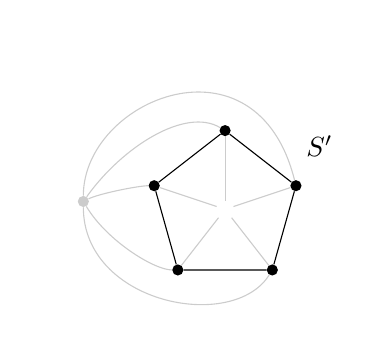
\begin{tikzpicture}[mid arrow/.style={
        postaction={ decorate, decoration={ markings, mark=at position 0.6 with { \arrow[black]{>>} } } } }]
        \draw[opacity=0] (-0.5, 0) ellipse (2cm and 1.5cm);
        \node[fill=white] at (1.2, 0.8) {$S'$};
        \node[inner sep=1mm] (c) at (0, 0) {$\core$};
        \node[circle, fill, scale=0.015cm] (l1) at (0, 1) { };
        \node[circle, fill, scale=0.015cm] (l2) at (0.9, 0.30) { };
        \node[circle, fill, scale=0.015cm] (l3) at (0.6, -0.77) {};
        \node[circle, fill, scale=0.015cm] (l4) at (-0.6, -0.77) {};
        \node[circle, fill, scale=0.015cm] (l5) at (-0.9, 0.30) {};
        \node[circle, fill, scale=0.015cm, opacity=0.2] (e) at (-1.8, 0.1) { };

        \draw[opacity=0.2] (e) .. controls +(0.2, 0.1) and + (-0.2, 0.0) .. (l5);
        \draw[opacity=0.2] (e) .. controls +(0.3, -0.5) and +(-0.3,0) .. (l4);
        \draw[opacity=0.2] (e) .. controls +(0.0,-1.3) and +(-0.5,-0.8) .. (l3);
        \draw[opacity=0.2] (e) .. controls +(0.0,+1.3) and +(-0.5,+2) .. (l2);
        \draw[opacity=0.2] (e) .. controls +(0.5,0.7) and +(-0.5, 0.3) .. (l1);

        \draw[opacity=0.2] (c) -- (l1);
        \draw[opacity=0.2] (c) -- (l2);
        \draw[opacity=0.2] (c) -- (l3);
        \draw[opacity=0.2] (c) -- (l4);
        \draw[opacity=0.2] (c) -- (l5);
        \draw (l1) -- (l2) -- (l3) -- (l4) -- (l5) -- (l1);
    \end{tikzpicture}
    \caption{The reductions $M+S$ and $\core+S'$ with $S=R_5+v$ for our specific choice of $S$ and $S'$.  }
    \label{fig:ring5k1}
\end{figure}

As expected, the only possible colorings of these reductions are 3-colorings like $\underline{c}abab$. There are five different 3-colorings of the ring $R_5$, we will be guaranteed of only one of them.

\begin{equation}
    \Phi^S = \{ 
        \underline{c}abab\;\;\text{or}\;\; 
        a\underline{c}bab\;\;\text{or}\;\;
        ab\underline{c}ab\;\;\text{or}\;\;
        aba\underline{c}b\;\;\text{or}\;\;
        abab\underline{c} \}.
\end{equation}

Taking everything together, we obtain the following guarantee on colorings in $\I$ and $\II$.

\begin{equation}
    \Phi^\star\; \cup \;\Phi^S \;\subset\; \I, \II.
\end{equation}

A special property of 3-colorings on $R_5$ is that there will always be a single vertex colored uniquely, we call this the \textit{marked vertex}. This vertex acts as a kind of 'pivot' to tell if two 3-colorings are \textit{adjacent}. These two concepts are key to the proof.

\begin{definition}
    The uniquely-colored vertex of a 3-coloring of $R_5$ is called the \emph{marked vertex}, indicated by an underline such as in $\underline{c}abab$.
\end{definition}

\begin{definition}
    Two 3-colorings of $R_5$ are called \emph{adjacent} if they have adjacent marked vertices, such as in $\underline{c}abab$ and $a\underline{c}bab$.
\end{definition}

Since we have guaranteed 3-colorings for both $\I$ and $\II$, we can split up our proof into 3 cases.

\begin{enumerate}
    \item $\I$ and $\II$ have an adjacent coloring ($\underline{c}abab$ and $a\underline{c}bab$).
    \item $\I$ and $\II$ have a non-adjacent coloring ($\underline{c}abab$ and $ab\underline{c}ab$).
    \item $\I$ and $\II$ have a coloring with the same marked vertex ($\underline{c}abab$ and $\underline{d}cbcb$). This always results in a common coloring.
\end{enumerate}

Therefore, we only need to consider the cases \circled{1} and \circled{2}. We will prove two lemma's to this end. Their relation is illustrated below.

\begin{equation*}
    \begin{aligned}
    \circled{2} \implies\; &\circled{1}\quad \text{or} \quad \text{common coloring} \quad\quad \text{(Lemma \ref{lem:r5_first})} \\
    &\downarrow \\
    &\circled{1} \implies\;\text{common coloring}\quad\quad \text{(Lemma \ref{lem:r5_second})}
    \end{aligned}
\end{equation*}

\begin{lemma}
    \label{lem:r5_first}
    If $\I$ and $\II$ have a non-adjacent coloring, then they either have an adjacent coloring or a common coloring.
\end{lemma}

\begin{proof}
Let two non-adjacent colorings $\I(\underline{c}abab)$ and $\II(ab\underline{c}ab)$ be given. Suppose that $v_3 \stackrel{bc}{\frown} v_5$ in $\II(ab\underline{c}ab)$. The two cases lead to the following.

\begin{equation}
    \label{eq:abcab}
    \begin{aligned}
        \II(ab\underline{c}ab) &=\scheme{a,b,c,a,b}{35b} \compat \II(abcdb), \\
        \II(ab\underline{c}ab) &= \scheme{a,b,c,a,b}{35b-} \compat \II(a\underline{c}bab).
    \end{aligned}
\end{equation}

The second case results in a coloring adjacent to $\I(\underline{c}abab)$. For the first case, we consider the coloring $\I({*}b{*}{*}b)$. The two adjacent ${*}$-colors must be different from each other and $b$, therefore we may assume that we have $\I({*}bcdb)$. The last ${*}$-color reveals 3 possibilities.

\begin{equation}
    \begin{matrix*}[l]
        \I(abcdb) \quad\quad =&\II(abcdb) \; \text{from (\ref{eq:abcab}),}  \\
        \I(cbc\underline{d}b) \;\; \text{adjacent to}&\II(ab\underline{c}ab), \;  \\
        \I(db\underline{c}db) \quad\quad =&\II(ab\underline{c}ab).
    \end{matrix*}
\end{equation}

Therefore we obtain either a common coloring or an adjacent coloring. Note that the pair of non-adjacent colorings we chose is the only unique one on $R_5$ (up to rotational symmetry).
\end{proof}

\begin{lemma}
    \label{lem:r5_second}
    If I and II have an adjacent coloring, then they have a common coloring.
\end{lemma}

\begin{proof}

Let two adjacent colorings $\I(\underline{c}abab)$ and $\II(a\underline{c}bab)$ be given. Suppose that $\chain{v_3}{v_5}{bd}$ in $\II(a\underline{c}bab)$. The two cases lead to the following.

\begin{equation}
    \label{eq:acdab}
    \begin{aligned}
        \II(a\underline{c}bab) &= \scheme{a,c,b,a,b}{35d} \compat \I(\underline{c}abab). \\
        \II(a\underline{c}bab) &= \scheme{a,c,b,a,b}{35d-} \compat \II(acdab).
    \end{aligned}
\end{equation}

The first case leads to a common coloring. For the second case,
we consider the coloring $\I(a{*}{*}a{*})$. We may again assume to have $\I(acda{*})$. Then the 3 remaining possibilities for the ${*}$-color are

\begin{equation*}
    \begin{matrix*}[l]
        \I(acdab) \quad =& \II(acdab), \;\text{from (\ref{eq:acdab})},\\
        \I(ac\underline{d}ac) \quad =\;\; \text{shifted $+2$}& \I(\underline{c}abab), \\
        \I(a\underline{c}dad) \quad =& \II(a\underline{c}bab).
    \end{matrix*}
\end{equation*}

If we do not obtain common colorings, we may repeat this procedure with $\II(a\underline{c}bab)$ and $\I(ac\underline{d}ac)$ to continously shift the marked vertex two to the right. The pattern that arises is illustrated in Figure \ref{table:ringpattern5} below.

\begin{figure}[!ht]
    \centering
    \begin{tabular}{c|ccccc:c}
         & $v_1$ & $v_2$  & $v_3$  & $v_4$ & $v_5$ & $v_1$  \\
        \hline
        1 & \I & \II &    &     &    & \I  \\
        2 &    & \II & \I &     &    &     \\
        3 &    &     & \I & \II &    &     \\
        4 &    &     &    & \II & \I &     \\
        5 &    &     &    &     & \I & \II \\
    \end{tabular}
    \caption{Marked vertices of $\I$ and $\II$ obtained by repetition of the earlier procedure.  Every step shifts the leftmost marked vertex two to the right. }
    \label{table:ringpattern5}
\end{figure}

At iteration 5, we obtain that $\II$ has the same marked vertex $v_1$ as $\I$. Therefore, by repetition we obtain that

\begin{equation}
    \II(\underline{c}abab) \rightarrow \II(aba\underline{c}b) \rightarrow \II(\underline{c}abab) = \I(\underline{c}abab).
\end{equation}

Therefore, adjacent colorings imply a common coloring for $\I$ and $\II$.

\end{proof}

Combining these two lemmas yields a guaranteed common ring coloring for $\I$ and $\II$ regardless of the case.

\end{proof}

In practice, the first step is to find the guaranteed 3-colorings from $M+S$ and $\core+S'$. Then, by conditioning on the marked vertex, we may need to use up to two ${*}$-colorings ($M$ and $\confg$ one each) depending on the Kempe-chains in the 3-colorings. Each ${*}$-coloring corresponds to a contraction of the ring vertices in $M+R_5$ or $\core+R_5$. Therefore, in the worst case, we have to color 4 smaller graphs before we can color $M+\confg$. In the ideal case only 2.